\subsection{Messung von Suszeptibilitäten}
Zur Bestimmung der Suszeptibilität wird die Brückenschaltung aus Abbildung
\ref{fig:schaltung} benötigt.
\begin{wrapfigure}{l}{6cm}
  \centering
  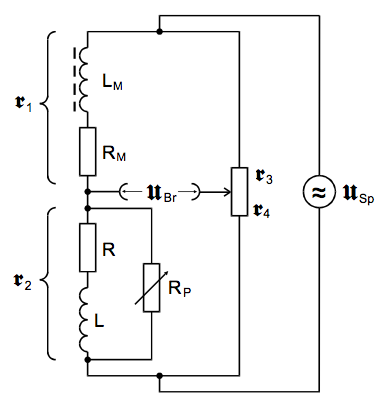
\includegraphics[width=5cm]{bilder/schaltung.png}
  \caption{Brückenschaltung zur Suszeptibilitätsbestimmung \cite{606}.}
  \label{fig:schaltung}
\end{wrapfigure}
Hierbei werden zwei gleiche Spulen verwendet, da die Messung auf einer
Induktivitätsdifferenz beruht. Der Widerstand $R_\su{p}$ wird verwendet,
um mögliche Unterschiede zwischen den Spulen auszugleichen. In die eine Spule wird das
zu untersuchende
Material eingesetzt. Dabei gibt es zwei Messmethoden. Bei der einen wird die
Brückenspannung $U_\su{Br}$ gemessen, welche entsteht, wenn die Probe in eine
Spule eingeführt wird. Für Frequenzen $\omega^2L^2 >>R^2$ gilt die Vereinfachung
\begin{equation}
 \chi (\omega \to \infty) = 4 \frac{F}{Q}\frac{U_\su{Br}}{U_\su{Sp}}
\end{equation}
mit $F$ als Spulenquerschnitt, $Q$ dem Querschnitt der Probe und $U_\su{Sp}$ der
Speisespannung.
Bei der anderen Methode werden die Brücken nach dem Einführen der Probe erneut
abgeglichen. Durch die dabei auftretende Differenz an den Einstellungen
lässt sich ebenfalls die Suszeptibilität mithilfe
\begin{equation}
 \chi = 2\frac{\Delta R}{R_3}\frac{F}{Q}
 \label{eqn:suszep}
\end{equation}
bestimmen. Hiebei ist $Q$ der Querschnitt der Probe und wird mit
\begin{equation}
  Q=\frac{M_\su{p}}{L\rho_\su{w}}
\end{equation}
berechnet. In diesem Experiment gilt $F = 86.6 \,\si{\square\milli\meter}$.
 $R_3$ beschreibt den Widerstand am Potentiometer, $M_\su{p}$ die Masse der Probe
und $\Delta R$ die Differenz der Einstellungen.

\subsection{Durchführung und Umsetzung}
Bei der Messung der Brückenspannung tritt ein Problem auf, da es zu Störspannungen
an den Ausgangsklemmen kommt, welche die Brückenspannung überdecken. Da die
Signalspannung monofrequent ist, kann ein Selektivverstärker genutzt werden,
um im Idealfall nur die gesuchte Brückenspannung durchzulassen. Dieser bietet
zusätzlich die Möglichkeit die Brückenspannung zu verstärken. Die Wirksamkeit
eines solchen Selektivverstärkers lässt sich durch die Güte $Q$ ausdrücken:
\begin{equation}
  Q = \frac{\nu_0}{\nu_+ - \nu_-}.
\end{equation}
\begin{figure}
  \centering
  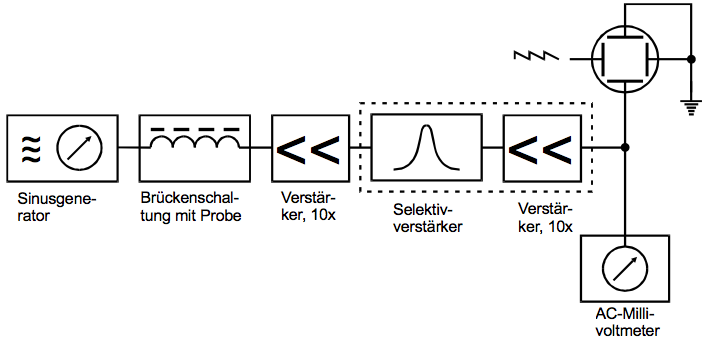
\includegraphics[width=10cm]{bilder/aufbau.png}
  \caption{Aufbau der Messapparatur \cite{606}.}
  \label{fig:aufbau}
\end{figure}
Ein möglicher Aufbau der Apparatur ist in Abbildung \ref{fig:aufbau} zu sehen.
Dabei erzeugt ein Sinusgenerator eine Wechselspannung von $1 \si{\volt}$ mit
einer Frequenz von $(20-40) \kHz$. Diese wird an den Eingang der Brückenschaltung
gelegt. $U_\su{Br}$ wird danach 10x vorverstärkt, bevor sie an den Selektivverstärker
gelegt wird.
Die dadurch gefilterte und verstärkte Spannung kann dann an den Buchsen "Resonance"
oder "Quadrature" abgenommen werden.

Zur Bestimmung der Suszeptibilität wird die Durchlassfrequenz des Selektivverstärkers
genau auf die Signalfrequenz gelegt. Dabei gilt $Q = 100$. Dazu wird ein Synthesizer
an den Verstärker angeschlossen. Mit einem Millivoltmeter werden 32 Spannungen
im Bereich $(20-40) \kHz$ mit den dazugehörigen Frequenzen an der Ausgangsspannung
$U_\su{A}$ abgelesen. Um das Maximum werden dabei $0.1 \kHz$ Schritte gewählt.
Daraufhin werden die Elemente $R_3 / R_4$ und $R_\su{p}$ auf eine möglichst niedrige
Spannungsdifferenz abgestimmt, Null ist aufgrund der übrig gebliebenen Störspannungen
nicht möglich. Diese Werte werden notiert.

Nun wird die Probe in die Zylinderspule eingeführt und die auftretende Brückenspannung
wird gemessen und notiert. Dann werden die Widerstände erneut abgestimmt.
Dieser Vorgang wird drei mal wiederholt. Zusätzlich müssen alle Verstärkungen
notiert werden. Am Ende werden noch die Massen $M_\su{Probe}$ der Proben und die Längen $l$ der
Gefäße gemessen.
